\documentclass[11pt]{article}

\usepackage[margin=1in]{geometry}
\usepackage{amsmath}
\usepackage{booktabs}
\usepackage{xcolor}
\usepackage{float}
\usepackage{algorithm}
\usepackage{algpseudocode}
\usepackage{tikz}
\usetikzlibrary{positioning,fit,arrows.meta}
\usepackage[hidelinks]{hyperref}

\definecolor{keepgreen}{HTML}{E5F2EA}
\definecolor{keepedge}{HTML}{1F6B45}
\definecolor{openred}{HTML}{F8E6E6}
\definecolor{openedge}{HTML}{8C2F2F}
\definecolor{dropgray}{HTML}{F2F1EE}
\definecolor{dropedge}{HTML}{8A8680}
\definecolor{sideamber}{HTML}{F6E4C0}
\definecolor{sideedge}{HTML}{8A6230}
\definecolor{ink}{HTML}{1C1B19}

\tikzset{
  evt/.style={draw, rounded corners=2pt, align=center, font=\scriptsize,
              inner sep=3pt, text=ink},
  kept/.style={evt, fill=keepgreen, draw=keepedge, line width=0.7pt},
  opened/.style={evt, fill=openred, draw=openedge, line width=0.7pt},
  dropped/.style={evt, fill=dropgray, draw=dropedge},
  sidel/.style={evt, fill=sideamber, draw=sideedge},
  flow/.style={-Stealth, thick, draw=ink!80}
}

\title{Feature-Attempt Hierarchies for Selecting\\ Coding-Agent Context and Attributing Its Cost}
\author{Kiran Kumar Kotari\\ \texttt{kkotari@cisco.com}}
\date{Working draft --- October 2026}

\begin{document}
\maketitle

\begin{abstract}
A coding agent that repairs one feature accumulates abandoned edits, resolved errors, and unrelated turns in the same trace.
A sliding window spends its budget on the newest tail of that trace, which can hide an older failure the agent still has to fix.
This thesis organizes the trace as a hierarchy: a feature at the root, an attempt under each edit, and a status on each tool failure.
The next prompt keeps the feature's instructions, the edit behind each open failure, and the open failure itself.
Superseded attempts and side threads remain in the hierarchy for accounting and stay out of the prompt.
The same hierarchy prices past model use as feature work, rework after the first failure, and side work.
On a five-trace pilot, this rule passes every context check.
A latest-error shortcut and a sliding window each pass two of five.
The pilot measures selection under a fixed budget.
It does not measure whether a model then repairs the code.
\end{abstract}

\section{Introduction}

Tool-using coding agents grow a trace of instructions, edits, and tool observations.
The next model call can carry only a limited history.
The usual control is a sliding window: keep the newest events that fit.
That control is simple, and it has a structural failure on repair work.
The event the agent most needs can be an older tool failure, while the newest events are a detour or a superseded attempt.

This thesis treats history as a hierarchy rather than a tape.
Each coding session has a feature.
Each edit opens an attempt.
A later edit marks the previous attempt superseded.
A tool failure is attached to the attempt that produced it and is marked open until a later successful compile resolves a syntax failure.
Side conversations sit on their own branch.
Selection then fills a fixed budget from that tree, newest open failure first, then the latest feature instruction, then the edit that caused each kept failure, then earlier instructions on the same feature.

The contribution is three parts:
\begin{enumerate}
  \item a feature, attempt, and open-failure hierarchy inferred from the trace;
  \item a budgeted selection rule that fills the next prompt from that hierarchy;
  \item a cost ledger that splits recorded model use into feature work, rework, and side work.
\end{enumerate}

Figure~\ref{fig:contrast} states the difference between the sliding window and this hierarchy.
Section~\ref{sec:trace} walks one trace from the pilot in full.
Section~\ref{sec:pilot} reports the five-trace comparison against the sliding window and a latest-error shortcut.

The pilot is a selection check on five handwritten traces.
Repair success and provider bills are unmeasured.

\section{Related work}

ContextWeaver organizes context by dependencies among steps~\cite{wu2026contextweaver}.
MemoTree follows the active path of a chat tree.\footnote{\url{https://github.com/thapakrish/memotree}}
This thesis reports a feature, attempt, and open-failure hierarchy, compared with a sliding window and a latest-error control.

\section{Method}
\label{sec:method}

\subsection{Trace and budget}

A case is a sequence of events.
Each event has an identifier, a turn, a kind, and text.
Kinds used by the hierarchy are user instructions, assistant edits, assistant analysis, and tool results.
An optional thread identifier separates the feature from side work.
When the identifier is absent, the event is treated as part of the feature.
A delivery contract sets a history budget in proxy units.
A proxy unit is one word or one punctuation mark from a regular expression.
It is not a provider tokenizer count and not a billed token.
The same contract carries a synthetic input and output price so past assistant calls can be converted into a dollar figure.
That figure is a ledger, not an invoice.

The context gate for a case is met when every required event is inside the selection and every known irrelevant event is outside it.
Required and irrelevant identifiers are evaluator labels.
Selectors do not read them.

\subsection{Hierarchy}

The root is the feature.
Walking the trace:
\begin{itemize}
  \item a side-thread event hangs under that thread and is out of scope for the feature prompt;
  \item an assistant edit closes the previous attempt as superseded and opens a new attempt;
  \item other feature events hang under the current attempt, except user instructions, which hang under the feature;
  \item a tool result that contains a syntax error, a traceback, a key error, a failing exit status, or an expected-versus-observed mismatch becomes an issue;
  \item a later tool result that runs \texttt{py\_compile} and reports success resolves open syntax issues.
\end{itemize}
Other open issues stay open.
A later edit does not by itself mean the earlier failure was fixed.

\subsection{Selection}

Algorithm~\ref{alg:select} fills the budget.
Open failures are considered from newest to oldest, so a tight budget prefers the current defect.
The latest feature instruction is next.
The edit that opened the attempt of each kept failure is next.
Earlier user instructions on the feature are last.
Those earlier instructions are where a constraint such as ``must preserve input order'' lives after the newest turn has stopped repeating it.
An event that would overflow the budget is skipped.
If nothing fits, selection fails closed.
The emitted list is restored to trace order so the model still sees a flat history.

\begin{algorithm}[H]
\caption{Feature-attempt context selection}
\label{alg:select}
\begin{algorithmic}[1]
\Require event trace $H$, budget $B$
\State $G \gets \textsc{BuildHierarchy}(H)$
\State $C \gets [\,]$
\State $F \gets$ feature events in $G$, excluding side threads
\State $U \gets$ latest user event in $F$, if any
\For{each open issue in $G$, from newest to oldest}
  \State append the issue event to $C$ if $C$ and that event fit in $B$
\EndFor
\State append $U$ to $C$ if it is new and fits
\If{$C$ is empty}
  \State \textbf{fail}: no active feature context
\EndIf
\For{each open issue whose event is in $C$}
  \State append that attempt's edit if it is new and fits
\EndFor
\For{each earlier user event in $F$, from newest to oldest}
  \State append it if it is new and fits
\EndFor
\State \Return events of $C$ in their original order in $H$
\end{algorithmic}
\end{algorithm}

\subsection{Cost}

For each assistant event with a recorded usage pair, synthetic cost is
\[
\frac{n_{\mathrm{in}}\cdot p_{\mathrm{in}} + n_{\mathrm{out}}\cdot p_{\mathrm{out}}}{10^{6}}.
\]
Feature cost sums assistant events whose parent is the feature or an attempt.
Side cost sums the others.
Rework is the feature portion of assistant events that occur after the first issue in the trace.
Missing usage makes that total unknown.
It is not recorded as zero.
The prices in the pilot are synthetic rates stored in the fixture, not a provider bill.

\begin{figure}[t]
\centering
\begin{minipage}[t]{0.46\textwidth}
\centering
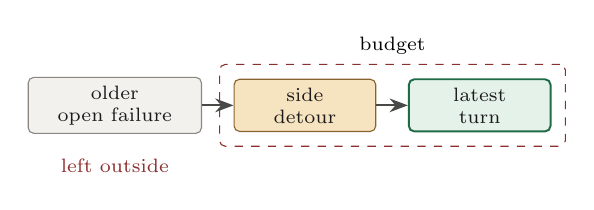
\begin{tikzpicture}[font=\scriptsize, node distance=4mm]
  \node[dropped, minimum width=22mm] (e1) {older\\open failure};
  \node[sidel, minimum width=18mm, right=of e1] (e2) {side\\detour};
  \node[kept, minimum width=18mm, right=of e2] (e3) {latest\\turn};
  \draw[flow] (e1) -- (e2);
  \draw[flow] (e2) -- (e3);
  \node[draw=openedge, dashed, rounded corners=2pt, fit={(e2) (e3)},
        inner sep=5pt, label={[font=\scriptsize]above:budget}] {};
  \node[font=\scriptsize, text=openedge, align=center, below=2mm of e1] {left outside};
\end{tikzpicture}

\vspace{2mm}
{\small (a) Sliding window. The budget covers the tail.}
\end{minipage}\hfill
\begin{minipage}[t]{0.50\textwidth}
\centering
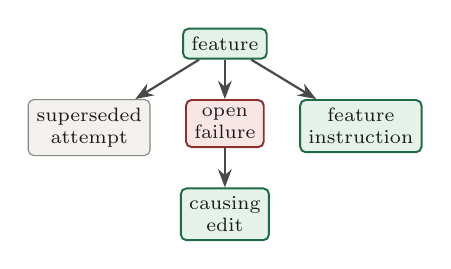
\begin{tikzpicture}[font=\scriptsize, node distance=5mm and 4mm]
  \node[kept] (root) {feature};
  \node[dropped, below left=of root] (old) {superseded\\attempt};
  \node[opened, below=of root] (err) {open\\failure};
  \node[kept, below right=of root] (ask) {feature\\instruction};
  \node[kept, below=of err] (edit) {causing\\edit};
  \draw[flow] (root) -- (old);
  \draw[flow] (root) -- (err);
  \draw[flow] (root) -- (ask);
  \draw[flow] (err) -- (edit);
\end{tikzpicture}

\vspace{2mm}
{\small (b) This hierarchy. The open failure and its edit stay.}
\end{minipage}
\caption{One repair trace under the two rules used in this thesis.
The sliding window spends the budget on the newest turns and leaves the open failure outside.
The hierarchy keeps the feature instruction, the edit that caused the open failure, and the failure.
The superseded attempt remains in the tree for the cost ledger and stays out of the prompt.}
\label{fig:contrast}
\end{figure}

\section{A worked trace}
\label{sec:trace}

Figure~\ref{fig:tree} is the catalog fixture after hierarchy construction.
The feature asks for an include-archived listing.
Attempt \texttt{e03} introduces a syntax error.
A later compile resolves that syntax issue, so the attempt is superseded.
Attempt \texttt{e07} compiles and then fails with \texttt{KeyError: 'title'} on an archived row that has no title.
That issue is open.
Events \texttt{e10} and \texttt{e11} are a side question about the Python version.
Event \texttt{e12} returns to the feature and states the missing rule: use the row's sku when the title is absent, preserve order, and do not mutate the input.

\begin{figure}[t]
\centering
\resizebox{\textwidth}{!}{%
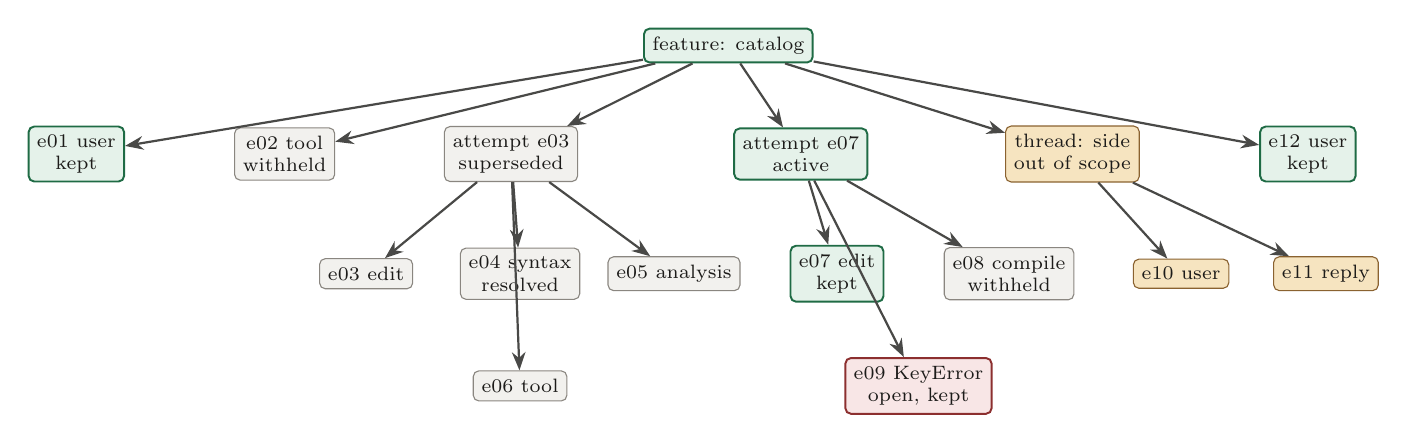
\begin{tikzpicture}[font=\scriptsize, x=1.15cm, y=0.95cm]
  \node[kept] (root) at (7.2,3.6) {feature: catalog};
  \node[kept] (e01) at (0.0,2.15) {e01 user\\kept};
  \node[dropped] (e02) at (2.3,2.15) {e02 tool\\withheld};
  \node[dropped] (a03) at (4.8,2.15) {attempt e03\\superseded};
  \node[kept] (a07) at (8.0,2.15) {attempt e07\\active};
  \node[sidel] (side) at (11.0,2.15) {thread: side\\out of scope};
  \node[kept] (e12) at (13.6,2.15) {e12 user\\kept};
  \node[dropped] (e03) at (3.2,0.55) {e03 edit};
  \node[dropped] (e04) at (4.9,0.55) {e04 syntax\\resolved};
  \node[dropped] (e05) at (6.6,0.55) {e05 analysis};
  \node[dropped] (e06) at (4.9,-0.95) {e06 tool};
  \node[kept] (e07) at (8.4,0.55) {e07 edit\\kept};
  \node[dropped] (e08) at (10.3,0.55) {e08 compile\\withheld};
  \node[opened] (e09) at (9.3,-0.95) {e09 KeyError\\open, kept};
  \node[sidel] (e10) at (12.2,0.55) {e10 user};
  \node[sidel] (e11) at (13.8,0.55) {e11 reply};
  \draw[flow] (root) -- (e01);
  \draw[flow] (root) -- (e02);
  \draw[flow] (root) -- (a03);
  \draw[flow] (root) -- (a07);
  \draw[flow] (root) -- (side);
  \draw[flow] (root) -- (e12);
  \draw[flow] (a03) -- (e03);
  \draw[flow] (a03) -- (e04);
  \draw[flow] (a03) -- (e05);
  \draw[flow] (a03) -- (e06);
  \draw[flow] (a07) -- (e07);
  \draw[flow] (a07) -- (e08);
  \draw[flow] (a07) -- (e09);
  \draw[flow] (side) -- (e10);
  \draw[flow] (side) -- (e11);
\end{tikzpicture}}
\caption{Inferred hierarchy for the catalog trace.
Green nodes are kept in the next prompt.
The red node is the open failure, and it is kept.
Gray nodes are withheld.
The amber branch is a side thread and is out of scope.
The prompt is e01, e07, e09, and e12, using 254 of 320 proxy units.}
\label{fig:tree}
\end{figure}

The selector emits four events, in trace order:
\begin{enumerate}
  \item \textbf{e01}, the original feature request, including the rule that the default listing still excludes archived items;
  \item \textbf{e07}, the active edit, which reads \texttt{row["title"]} and adds no fallback;
  \item \textbf{e09}, the open \texttt{KeyError};
  \item \textbf{e12}, the latest instruction, which names the sku fallback.
\end{enumerate}
The resolved syntax error, the passing compile, and the side thread stay in Figure~\ref{fig:tree} so the cost ledger can still see them.
They are absent from the prompt.
Workspace files are available to the agent as files.
They are not pasted into the history budget.

\section{Pilot study}
\label{sec:pilot}

\subsection{Fixtures and protocol}

Five handwritten fixtures share one protocol.
Each has a single continuation checkpoint, a history budget of 320 proxy units, and a synthetic price of \$2 per million input units and \$8 per million output units.
Selectors see the public events only.
The gate uses private required and irrelevant identifiers stored beside the fixture.

The five situations are the ones this hierarchy is meant to handle:
\begin{itemize}
  \item a long package-list detour that pushes an older cache \texttt{KeyError} outside a recent-history window;
  \item an ordering constraint stated in an early user turn and absent from the latest turn;
  \item two open shipping failures, a missing name and a reversed order, with no successful compile between them;
  \item a refund mismatch written as expected versus observed, without the word ``error'';
  \item a resolved syntax error beside a later open \texttt{KeyError}, plus a side thread.
\end{itemize}

No selector calls a model.
No selector executes the fixture project.
Repair success, latency, and provider cost are therefore empty on every row.

\subsection{Baselines}

The pilot compares Algorithm~\ref{alg:select} with the two controls from Section~2.
The chronological suffix keeps the newest events that fit the budget.
The latest-error control keeps one error-like tool result and the latest user turn.
Both are selection rules on the same events and the same budget.
They do not use the hierarchy.

\subsection{Results}

Table~\ref{tab:gates} is the aggregate.
The hierarchy passes 5 of 5 gates.
The chronological suffix passes 2 of 5.
The three misses are the long detour, the catalog side thread, and the refund trace, where the window still contains irrelevant events.
The cache case is the sharp one.
Its current context is the smallest of the five, 47 proxy units, because the package list does not fit and the older \texttt{KeyError} falls outside the window.
That check fails.
The hierarchy context is larger, and it keeps the \texttt{KeyError}, so the same case passes.
This is a failed context check.
No model was run to show that the repair itself stays unsolved.
The latest-error control also passes 2 of 5.
It misses the early ordering constraint, the second open shipping failure, and the refund mismatch, whose text does not look like a traceback.
The hierarchy keeps every open failure, so both shipping defects stay, and it keeps the earlier instruction, so the ordering constraint stays.

\begin{table}[t]
\centering
\caption{Context checks on five fixtures.
A pass means required events are kept and known irrelevant events are excluded.
Proxy units are regular-expression counts, not provider tokens.}
\label{tab:gates}
\small
\begin{tabular}{@{}lrrr@{}}
\toprule
Selector & Gate & Mean units & Mean discarded \\
\midrule
Chronological suffix & 2/5 & 198.4 & 201.4 \\
Latest error and latest user & 2/5 & 81.4 & 318.4 \\
Feature-attempt hierarchy & 5/5 & 172.2 & 227.6 \\
\bottomrule
\end{tabular}
\end{table}

Table~\ref{tab:cost} is the ledger for past assistant calls on the same traces.
Each total matches the fixture's private synthetic reference.
Rework is large on the catalog and shipping traces because most feature model use sits after the first failure.
Side work is a small, separate number where a detour exists, and zero where the trace stays on one feature.
The hierarchy decides what the next prompt repeats.
The ledger attributes past model use to the feature, to rework, and to side work.
The prices are the fixture rates.

\begin{table}[t]
\centering
\caption{Synthetic past model cost in US dollars, split by the hierarchy.
Rework is the feature portion after the first issue.
These are not provider invoices.}
\label{tab:cost}
\small
\begin{tabular}{@{}lrrr@{}}
\toprule
Fixture & Feature & Rework & Side \\
\midrule
Catalog, include archived & 0.006200 & 0.004600 & 0.000260 \\
Refund sign position & 0.003960 & 0.002360 & 0.000260 \\
Compact display order & 0.002940 & 0.001540 & 0.000000 \\
Shipping, two open failures & 0.005720 & 0.004060 & 0.000000 \\
Cache expiry, long detour & 0.001500 & 0.000000 & 0.000260 \\
\bottomrule
\end{tabular}
\end{table}

The hierarchy is the only selector that passes every fixture.
That is evidence about this gate on these five traces.
It is not evidence that a coding agent resolves more issues.

\section{Conclusion}

A feature-attempt hierarchy tells a coding agent what to keep under a tight budget and what the feature has already cost.
Keep the feature's instructions, the edit behind each open failure, and the open failure.
Leave superseded attempts and side threads in the tree for the ledger, and leave them out of the prompt.
On five fixtures that rule passes every context check, where a sliding window and a latest-error shortcut each pass two.
The result is a selection result.
Repair outcomes and provider bills remain to be measured.
The same tree can root on an idea or a topic instead of a coding feature: keep that thread, drop side talk, and count the cost.
The evidence in this paper is five coding traces.
A claim about ideas or topics is a separate study.

\begin{thebibliography}{9}
\bibitem{wu2026contextweaver}
Y.~Wu, Y.~Zhang, S.~Ghosh, S.~Basu, A.~Deoras, J.~Huan, and G.~Gupta.
ContextWeaver: Selective and dependency-structured memory construction for LLM agents.
arXiv:2604.23069, 2026.
\end{thebibliography}

\end{document}
